% Copyright (c) Eclipse Arrowhead Project
%
% This program and the accompanying materials are made available under the
% terms of the Eclipse Public License 2.0 which is available at
% http://www.eclipse.org/legal/epl-2.0.
%
% SPDX-License-Identifier: EPL-2.0

\documentclass[a4paper]{arrowhead}

\usepackage[yyyymmdd]{datetime}
\usepackage{enumitem}
\usepackage{etoolbox}
\usepackage[utf8]{inputenc}
\usepackage{multirow}

\renewcommand{\dateseparator}{-}

\begin{document}

%% Arrowhead Document Properties
\ArrowheadTitle{Eclipse Arrowhead Core Documentation Reference}
\ArrowheadType{Reference Architecture}
\ArrowheadTypeShort{RA}
\ArrowheadVersion{0.1}
\ArrowheadDate{\today}
\ArrowheadAuthor{Emanuel Palm}
\ArrowheadStatus{Work in Progress}
\ArrowheadContact{emanuel.palm@pinterop.se}
\ArrowheadFooter{\href{www.arrowhead.eu}{www.arrowhead.eu}}
\ArrowheadSetup
%%

%% Front Page
\begin{center}
  \vspace*{1cm}
  \huge{\arrowtitle}

  \vspace*{0.2cm}
  \LARGE{\arrowtype}
  \vspace*{1cm}
  \vspace*{\fill}

  % \includegraphics[scale=1.5]{path/to/image}

  \vspace*{1cm}
  \vspace*{\fill}

  \begin{abstract}
    This document establishes how to read and write the documentation for entities of the \textit{Eclipse Arrowhead}, a framework designed to help create highly dynamic industrial systems.
    It also provides guidelines regarding the production of \textit{conformant} documentation, as well as describing how significant documentation can be ratified.
  \end{abstract}

  \vspace*{1cm}
\end{center}
\newpage
%%

%% Table of Contents
\tableofcontents
\newpage
%%

\section{Introduction}
\label{sec:introduction}
% Copyright (c) 2021 Eclipse Arrowhead Project
%
% This program and the accompanying materials are made available under the
% terms of the Eclipse Public License 2.0 which is available at
% http://www.eclipse.org/legal/epl-2.0.
%
% SPDX-License-Identifier: EPL-2.0

We expect the automation systems of today to keep becoming more and more computerized, digitized and interconnected.
By this we mean that more aspects of and surrounding automation machines will be handled by computers, more information will be made available to those computers and, finally, comparatively more such computers will be given the opportunity to collect, communicate and act on that information.
Manufacturing, transportation, energy distribution, medicine, recycling, as well as all other industrial sectors concerned with automation we believe will be affected by this development.
It will lead to increased automation efficiency and flexibility, as machines become able to perform more of the work traditionally assigned to humans.
However, it will also lead to new magnitudes of complexity, not the least because of the renewed incentive to use more and more of these highly communicative machines.

The \GlossaryHyperRef{framework-arrowhead}{\textit{Arrowhead framework}} is designed to address this explosion of complexity.
It provides a foundation for \GlossaryHyperRef{communication-service-oriented}{\textit{service-oriented communication}} \cite{mackenzie2006reference} between automation systems and other computers, such that interoperability, security, safety, performance, and other major concerns can be addressed efficiently and effectively.
It notably allows for \GlossaryHyperRef{system}{system} \GlossaryHyperRef{capability}{capabilities} to be \GlossaryHyperRef{description}{described}, shared and exploited dynamically by communicating \GlossaryHyperRef{device}{devices}.

In this document, we, the Eclipse Arrowhead project, present an authoritative set of concept definitions, meant to serve as the fundamental language for discussions about and the modeling of Arrowhead-based system \GlossaryHyperRef{design}{designs}.
These definitions exist to help mitigate compatibility and consistency issues in \GlossaryHyperRef{software}{software}, tooling, \GlossaryHyperRef{model}{models}, documentation and all other things of relevance to the Arrowhead framework.

\subsection{Primary Audiences}
\label{sec:introduction:audiences}

This document is being written and maintained for all who need precise and rigorous definitions of important Arrowhead concepts, which we understand to likely include the following groups:

\begin{itemize}
\item \GlossaryHyperRef{developer}{Developers} of Arrowhead systems.
\item \GlossaryHyperRef{researcher}{Researchers} concerned with analyzing or refining the Arrowhead framework or Arrowhead systems.
\item \GlossaryHyperRef{builder}{Builders}, \GlossaryHyperRef{maintainer}{maintainers} and \GlossaryHyperRef{operator}{operators} of Arrowhead systems.
\item \GlossaryHyperRef{acquirer}{Acquirers}, \GlossaryHyperRef{owner}{owners} and \GlossaryHyperRef{supplier}{suppliers} of Arrowhead systems.
\item Advanced \GlossaryHyperRef{user}{users} of Arrowhead systems.
\end{itemize}

\subsection{Scope}
\label{sec:introduction:scope}

This document is intended to clearly define all technical concepts of fundamental importance to the Arrowhead framework.
It does not specify how Arrowhead-based automation systems ought to be designed.
This makes its purpose analogous to that of a dictionary.
Dictionaries define words.
They may give examples of how certain words may be used, but they do not require that those words be used for any particular purposes.
This document provides an Arrowhead vocabulary other documents or models may use to express software-centric automation system designs.

The concepts presented here are meant to be useful as a resource for advanced Arrowhead framework learners, as well as to serve as foundation for other documentation and modeling efforts.
This document does \textit{not} define an Arrowhead profile for SysML \cite{omg2019sysml}, or any other modeling language.
For those interested in using this document for software-architectural purposes, a description of how it can be used as a \GlossaryHyperRef{modelmeta}{metamodel} in the context of an ISO/IEC/IEEE 42010 \GlossaryHyperRef{kind-model}{model kind} is provided in Section \ref{sec:conformance:iso42010}.

\newpage

\subsection{Notational Conventions}
\label{sec:introduction:conventions}

The following conventions regarding diagrams depicting graphs, references and requirements are adhered to throughout this document.

\subsubsection{Graph Diagrams}

A box with a solid border and a name inside it denotes a named \GlossaryHyperRef{entity}{entity}, useful for representing any Arrowhead \GlossaryHyperRef{artifact}{artifact} or \GlossaryHyperRef{stakeholder}{stakeholder}.
A named arrow between boxes denotes the \GlossaryHyperRef{relationship}{relationship} implied by the name.
Relationship names should be defined, or have their definitions referred to, in relation to the figures they are used in.
Exceptions are acceptable if the implications of a given name can be considered obvious.
The following five relationship names must be understood to always be defined:

\begin{enumerate}
\item \textit{refers to}, which means that the origin entity knows of or names the target entity;
\item \textit{conforms to}, which means that the origin entity \textit{refers to} the target entity and satisfies all \GlossaryHyperRef{constraint}{constraints} implicitly and/or explicitly associated with that target entity;
\item \textit{extends}, which means that the origin entity \textit{conforms to} the target entity and inherits all of its relationships;
\item \textit{is}, which means that the origin entity \textit{extends} the target entity and is member of a group named after that target entity; and, finally,
\item \textit{has}, which means that the origin entity \textit{refers to} and owns the target entity, where ownership entails exclusive access to and control over the owned entity.
\end{enumerate}

\paragraph{Quantifiers}
If a named arrow has an associated positive integer or range, which we refer to as a \textit{quantifier}, the relation is to be considered as extending to the number of distinct entities indicated by that integer or range.
No quantifier being present implies a quantity of 1.
A range is denoted by $x..y$, where $x$ and $y$ are integers and $0 \leq x < y$.
If $y$ is substituted by $*$, the range must be understood to extend infinitely from $x$ (e.g. ``$1..*$'').

\paragraph{Groups}
A box with a dotted border represents a \textit{group}.
The entities explicitly placed within the box may or may not represent all entities of that group.
If a relationship extends to or from a group, rather to any entity inside that group, the relationship must be understood to extend to or from all entities inside that group.

\paragraph{Combined Arrows}
If two or more arrows are combined such that their source or target end is shared, a difference is made if a quantifier is closest to a shared or non-shared arrow part.
If it is closest to a shared part, the quantity must be understood to apply to the arrows of the combination collectively.
For example, if an arrow extends from one entity to three other entities and the quantifier is ``$0..1$'' at the shared part, the relationship extends to only zero or one of the three entities.
If a quantifier is closest to a non-shared part, the quantifier must be understood to only apply to the relationship of that arrow only.
Combined arrows may have quantifiers both at their shared and non-shared parts, which are associated with the quantifiers $0..*$ and $1$, respectively, if not explicitly specified.
If an arrow extends to or from a group, that arrow must be considered as a shared part of a set of combined arrows.

\subsubsection{References}

Square brackets around numbers (e.g. \cite{delsing2017iot}) are references to the reference list in Section \ref{sec:references}.
The number within the brackets of any given reference corresponds to the entry with the same number in the reference list.

References within this document are hyperlinked, which means that those reading it electronically can click the references and immediately be taken to their targets.
Special treatment is given to references targeting Section \ref{sec:glossary}, the \nameref{sec:glossary}.
These are displayed as regular text rendered with blue color.

\subsubsection{Requirements}

Use of the terms \textbf{must}, \textbf{must not}, \textbf{should}, \textbf{should not} and \textbf{may} are to be interpreted as follows when used in this document: \textbf{must} and \textbf{must not} denote absolute requirements and prohibitions, respectively; \textbf{should} and \textbf{should not} denote recommendations that should be deviated from only if special circumstances make it relevant; and, finally, \textbf{may} denotes something being truly optional.

\subsection{Relationships to Other Documents}
\label{sec:introduction:relationships}

When this \GlossaryHyperRef{model-reference}{reference model} was produced, care was taken to reuse or build upon the concepts presented in the following works, in order of precedence:

\begin{enumerate}

\item \textbf{IoT Automation: Arrowhead Framework} (IoTA:AF) \cite{delsing2017iot}, which significantly includes an overview of the \textit{local automation cloud} concept in its second chapter, as well as the \textit{Arrowhead framework architecture} in its third chapter.
The book most significantly represents the state of the Arrowhead framework up until it was written.
Even though the framework has evolved since then, it still represents the most comprehensive view of the framework.
While the strictly architectural aspects of IoTA:AF are outside the scope of this document, the two mentioned chapters contain several definition with a high degree of relevance.

\item \textbf{ISO/IEC/IEEE 42010 Systems and software engineering — Architecture description} (ISO42010) \cite{iso42010}, which outlines a standardized approach to structuring architectural documents and models.
The standard is adhered to in the sense that the definitions of this document are meant to be useful as a metamodel part of a so-called \GlossaryHyperRef{kind-model}{\textit{model kind}}, as defined by the standard.
No claim of conformance to the standard is made for this document on its own.

\item \textbf{Reference Model for Service Oriented Architecture} (SOA-RM) \cite{mackenzie2006reference}, which provides a standardized definition of Service-Oriented Architecture (SOA).
As communication between \GlossaryHyperRef{system}{systems} of the Arrowhead framework is understood to follow this paradigm, it becomes particularly relevant to consider.

\item \textbf{Reference Architecture Model Industrie 4.0} (RAMI4.0) \cite{adolphs2016reference}, which outlines an ontological and architectural view of \GlossaryHyperRef{industry40}{\textit{Industry 4.0}}.
The document may be seen as a predecessor to, or major influence on, the conceptual aspects of the Arrowhead framework.
In particular, the document describes how to model and design communicating industrial systems such that key Industry 4.0 characteristics can be facilitated, such as high degrees of dynamicity and interoperability.
However, as RAMI4.0 is a reference \textit{architecture} rather than a reference \textit{model}, we have only been concerned with what concepts it defines and what problems it frames.
This delimitation excludes its ``architectural layers'', ``life-cycle \& value-stream'' phases and ``hierarchical levels'', as well as the abstract design of its ``asset administrative shell''.
These excluded aspects are neither condemned nor endorsed by this document.
They are simply outside its scope.

\end{enumerate}

Only conformity with IoTA:AF and ISO42010 is observed strictly, which means that concept definitions presented here may diverge from those of the other two works.
All significant terminology differences are noted in the glossary of Section \ref{sec:glossary}, which briefly defines all concepts of relevance to this document.

\subsection{Section Overview}
\label{sec:introduction:sections}

The remaining sections of this document are organized as follows:
\vspace*{2mm}
\begin{itemize}[leftmargin=2cm,rightmargin=0pt,labelwidth=2cm,labelsep=0pt,itemindent=0pt,parsep=0.1cm,topsep=0.1cm,align=left]

\item[Section \ref{sec:introduction}]
This section.

\item[Section \ref{sec:arrowhead}]
A formal overview of Arrowhead, describing how its core concepts relate to each other.
The section also serves to provide a workable summary of the framework and to prepare readers for better understanding Section \ref{sec:concepts}.

\item[Section \ref{sec:concepts}]
A formal description of the primary concepts of Arrowhead.
Each of its subsections is concerned with primary concept, ranging from entities to systems-of-local-clouds.

\item[Section \ref{sec:conformance}]
A list of requirements, meant to help determine if a document or model referring to the concepts of this document can be considered conformant.
A special subsection on ISO/IEC/IEEE 42010 conformance is also provided.

\item[Section \ref{sec:glossary}]
Lists all significant terms and abbreviations presented in this document in alphabetical order.

\item[Section \ref{sec:references}]
Lists references to publications referred to in this document.

\item[Section \ref{sec:revision}]
Records the history of changes made to this document.

\end{itemize}


\section{Overview}
\label{sec:overview}
% Copyright (c) 2021 Eclipse Arrowhead Project
%
% This program and the accompanying materials are made available under the
% terms of the Eclipse Public License 2.0 which is available at
% http://www.eclipse.org/legal/epl-2.0.
%
% SPDX-License-Identifier: EPL-2.0

The \GlossaryHyperRef{framework-arrowhead}{Arrowhead framework}, which is illustrated in Figure \ref{fig:framework}, consists of two subframeworks: a \GlossaryHyperRef{framework-idea}{framework of ideas} and a \GlossaryHyperRef{framework-software}{framework of software}.
The framework of ideas formulates and frames the \GlossaryHyperRef{domain-problem}{\textit{problem domain}} the framework of software is meant to help address.
By this we mean that the framework of ideas presents the \GlossaryHyperRef{assumption}{assumptions}, \GlossaryHyperRef{concept}{concepts}, \GlossaryHyperRef{value}{values} and \GlossaryHyperRef{practice}{practices} that should be applied when \GlossaryHyperRef{specification}{specifying} \GlossaryHyperRef{architecture}{architectural} or other technical documentation and when \GlossaryHyperRef{implementation}{implementing} any kinds of Arrowhead systems or components.

\begin{figure}[ht!]
  \centering
  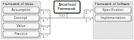
\includegraphics[scale=0.9]{figures/framework}
  \caption{
    The two subframeworks of the Arrowhead framework, concerned with \textit{ideas} and \textit{software}.
    The specifications and implementations of the software framework must conform to the assumptions, concepts, values and practices of the idea framework.
    The concepts of the idea framework are outlined in this document.
  }
  \label{fig:framework}
\end{figure}

This document is part of Arrowhead's framework of ideas.
As such, it is primarily concerned with defining concepts.
However, before we move on to consider our overview those concepts, we will first present a few examples of other key framework ideas.\footnote{
  At the time of writing, the best source of assumptions, values and practices of the Arrowhead framework is Jerker Delsing's book \textit{{IoT} Automation: Arrowhead Framework} \cite{delsing2017iot}.
  The \GlossaryHyperRef{project-eclipse-arrowhead}{Eclipse Arrowhead project} may publish other works of relevance in the future.
}
It is, for example, \textit{assumed} that the framework may be applied in contexts where the primary activity is markedly physical, such as in transportation, mining, manufacturing, electricity generation, healthcare, and so on.
One of the system characteristics \textit{valued} by the framework is \textit{resilience}, or the expectation that every system should do its outmost to mitigate and recover from degradations, failures or other contingencies that may affect its ability to perform its designated tasks.
Finally, one of its \textit{recommended practices} is that every system-of-systems should be thoroughly documented at every level, from its smallest components up to its most high-level interactions.

The rest of this section gives an overview of the most fundamental concepts of the framework.
It is meant to prepare you for the next section, where the same concepts, and other supporting concepts, are presented in greater detail.

\subsection{Stakeholders and Artifacts}

There are two kinds of members of the world of Arrowhead, (1) \GlossaryHyperRef{stakeholder}{stakeholders} and (2) \GlossaryHyperRef{artifact}{artifacts}, as depicted in Figure \ref{fig:world}.
The former denotes a \GlossaryHyperRef{person}{person} or \GlossaryHyperRef{organization}{organization} engaged in an Arrowhead enterprise, while the latter is any thing or object, tangible or intangible, that could be relevant to consider as part of such an enterprise.
Stakeholders \GlossaryHyperRef{owner}{own}, \GlossaryHyperRef{supplier}{supply}, \GlossaryHyperRef{developer}{develop}, \GlossaryHyperRef{operator}{operate}, and \GlossaryHyperRef{user}{use} artifacts, among many other possible activities.
It is their business needs and ambitions that govern what and how Arrowhead artifacts are employed.

\vfill

\begin{figure}[ht!]
  \centering
  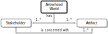
\includegraphics[scale=0.9]{figures/world}
  \caption{
    The two kinds of members of the Arrowhead world: stakeholders and artifacts.
  }
  \label{fig:world}
\end{figure}

\subsection{Devices, Systems and Services}

The most essential types of artifacts in the world of Arrowhead are (1) \GlossaryHyperRef{device}{hardware devices}, (2) \GlossaryHyperRef{system}{software systems} and (3) \GlossaryHyperRef{service}{services}, all shown in Figure \ref{fig:device-system-service}.
\textit{Hardware devices}, or just \textit{devices}, are physical machines, such as servers, robots or tools, that are able to maintain, or \GlossaryHyperRef{hosting-system}{\textit{host}}, \textit{software systems}.
A software system, or just \textit{system}, is a \GlossaryHyperRef{communication}{communicating} \GlossaryHyperRef{instance-software}{software instance} that \GlossaryHyperRef{provision-service}{provides} \textit{services}.
Every service represents a set of tasks a system can perform for other systems or for its stakeholders.
When a system or stakeholder makes use of a service, it is said to \GlossaryHyperRef{consumption-service}{\textit{consume}} it.

\vfill

\begin{figure}[ht!]
  \centering
  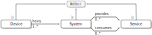
\includegraphics[scale=0.9]{figures/device-system-service}
  \caption{
    Hardware devices \textit{host} software systems, which \textit{consume} and/or \textit{provide} services.
  }
  \label{fig:device-system-service}
\end{figure}

\vfill

Every service represents one area of concern its hosting system can address.
Examples of such areas of concern could be generating financial statements, replacing propellers on drones, manufacturing bolts or measuring humidity.
A service providing control over a door could, for example, make it possible to check if the door is open, to open it and to close it.
Each such activity of every service is represented by one \GlossaryHyperRef{operation-service}{service operation}, which we will consider more in the next section.

\subsection{Service Provision and Consumption}

As we have already established, \GlossaryHyperRef{communication}{communication} between systems is formulated in terms of the \GlossaryHyperRef{provision-service}{provision} and \GlossaryHyperRef{consumption-service}{consumption} of \GlossaryHyperRef{service}{services}.
\GlossaryHyperRef{system}{Systems} may \textit{provide} services, which other systems can \textit{consume} by sending \GlossaryHyperRef{message}{messages} to their \GlossaryHyperRef{operation-service}{operations}, as depicted in Figure \ref{fig:service-consumption}.

\vfill

\begin{figure}[ht!]
  \centering
  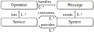
\includegraphics[scale=0.9]{figures/service-consumption}
  \caption{
    Systems consume services by sending messages to the providers of those services.
    Those providers then pass on the messages they receive to their service operations, which interpret and handle them.
  }
  \label{fig:service-consumption}
\end{figure}

\vfill

Also \GlossaryHyperRef{person}{persons} can consume services, even though it is not explicitly depicted in Figure \ref{fig:service-consumption}.
This, however, requires that a \GlossaryHyperRef{interface-human}{human interface} is attached to the providing system, or that another system with such an interface can act as \GlossaryHyperRef{proxy}{proxy}.
The human interface enables the person, via its buttons, prompts or other elements, to send messages to the services in question, just as a regular system would.

When a providing system receives a message from a consuming system or person, it passes it on to the service operation specified in that message, as described in Sections \ref{sec:concepts:service} and \ref{sec:concepts:interface}.
The operation receiving the message will then handle it by performing whatever action it describes, given that the message is \GlossaryHyperRef{message-valid}{valid} and \GlossaryHyperRef{message-permitted}{permitted}.
This handling may entail sending additional messages to other systems, starting or stopping various kinds of automation routines, reading from sensors, electronically signing contracts, sending notifications to an \GlossaryHyperRef{operator}{operator}, sending one or more messages back to the sender, among many other possible examples.

\subsection{System Composition}
\label{sec:overview:system-composition}

\GlossaryHyperRef{system}{Systems} will typically \GlossaryHyperRef{consumer-service}{consume services} because it is a necessary part of executing the tasks they were designed to perform.
Consider, for example, a scenario in which a number of automated guided vehicles, each of which is a system, are to move items around a factory as directed by a scheduling system.
As the scheduling system does not have wheels, engine or other necessary sensors and actuators, it cannot physically move any items by itself. 
Likewise, the individual vehicles are not capable of themselves deciding what needs to be taken to what location.
However, when these different systems cooperate by consuming each others' services, they become able to do things none of them could by themselves.
The combination of scheduling system and vehicles becomes able to plan, track and execute the moving of items.
When systems consume each other's services in this manner, they form a so-called \GlossaryHyperRef{system-of-systems}{system-of-systems}.
Such a system-of-systems is often capable of performing activities none of its constituent \GlossaryHyperRef{subsystem}{subsystems} could perform on its own.

As depicted in Figure \ref{fig:systems-of-systems}, there are different kinds of systems-of-systems with their own characteristics.
There are \GlossaryHyperRef{cloud}{clouds} and \GlossaryHyperRef{system-of-clouds}{systems-of-clouds}, as well as \textit{local} and \textit{virtual} variants of both.

\vfill

\begin{figure}[ht!]
  \centering
  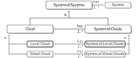
\includegraphics[scale=0.9]{figures/systems-of-systems}
  \caption{
    The different kinds of \textit{systems-of-systems}, each of which consists of a number of \textit{systems} that consume each others' services.
    Clouds are systems-of-systems with \textit{boundaries} and \textit{resource pools}, while systems-of-clouds combine multiple clouds.
  }
  \label{fig:systems-of-systems}
\end{figure}

\vfill

When a system-of-systems has at least one \GlossaryHyperRef{boundary-cloud}{boundary} and at least one pool of \GlossaryHyperRef{resource}{resources}, we refer to it as a \textbf{cloud}.
Boundaries may be formed via access control policies, firewalls, gateway systems, physical separation, among many other possible examples.
Pools of resources may consist of mining equipment, \GlossaryHyperRef{unit-compute}{compute units}, sand, or whatever else is used by the cloud in question to render its services.
Because the Arrowhead framework is highly concerned with physical automation processes, we distinguish \GlossaryHyperRef{cloud-local}{local clouds} from \GlossaryHyperRef{cloud-virtual}{virtual clouds}.

The \textbf{local cloud} has \GlossaryHyperRef{boundary-local}{local boundaries} and \GlossaryHyperRef{resource-local}{local resources}, which means that it must be associated with a physical location.
Examples of local clouds could be smelting stations, drone control towers, assembly lines, power distribution centers, or the components of a satellite.
Whether it be ore, drones, parts, power cables or a complex mesh of all those things, the resources of these example clouds are all markedly \textit{physical}.
Because of their physicality, it matters \textit{where} the clouds are physically located.
Since physical isolation is a form of physical boundary, each of them has both at least one local boundary and at least one local resource.

On the other hand, a \textbf{virtual cloud} has only \GlossaryHyperRef{boundary-virtual}{virtual boundaries} and \GlossaryHyperRef{resource-virtual}{virtual resources}, which means that the values produced by the cloud are not tied to its physical location.
This is the kind of cloud that underpins much of the modern Internet.
A few companies let out virtual compute, storage and network resources, which their clients rent to provision their own virtual clouds and provide their own virtual services.
A virtual cloud could provide services for forecasting, analysis, design, planning, communication, or digital entertainment, among other possible examples.

Individual clouds may be interconnected to former even larger systems-of-systems, which we then refer to as \textbf{systems-of-clouds}.
The individual clouds may be owned and operated by different departments, subdivisions or teams at the same company, or even by different legal entities.
Some of them may be local, while other may be virtual.
Examples of systems-of-clouds may be a set of weather stations operated by the same company, the robots of distinct collaborating companies at a mining site, or the carriers of a supply chain.
When a system-of-clouds contain only local clouds, we refer to it as a \GlossaryHyperRef{system-of-local-clouds}{systems-of-local-clouds}.
Likewise, a system-of-clouds with only virtual clouds constitute a \GlossaryHyperRef{system-of-virtual-clouds}{systems-of-virtual-clouds}.


\section{Formats}
\label{sec:formats}
% Copyright (c) 2021 Eclipse Arrowhead Project
%
% This program and the accompanying materials are made available under the
% terms of the Eclipse Public License 2.0 which is available at
% http://www.eclipse.org/legal/epl-2.0.
%
% SPDX-License-Identifier: EPL-2.0

TODO

The three major categories of formats in which Arrowhead documentation can be expressed.
The categories are (1) print, (2) interactive, and (3) semantic.

Print documentation is concretely rendered as documents that can be printed out on paper.
Interactive documentation is presented in the form of an interactive computer application, such as a website or a plugin in a development environment.
Finally, semantic documentation exists as machine-readable definitions that can be used as input to produce other forms of documentation or generate other artifacts of interest (such as parts of computer programs).

As this document is a \textit{Reference Architecture}, it does not specify how to realize any of these three formats.
So-called \textit{Concrete Architecture} (CA) documents would have to be specified for each format of interest.
As this document is produced in LaTeX, I will write such a CA-document for LaTeX/print documentation at some later point.

\section{Framework Descriptions}
\label{sec:framework}
% Copyright (c) 2021 Eclipse Arrowhead Project
%
% This program and the accompanying materials are made available under the
% terms of the Eclipse Public License 2.0 which is available at
% http://www.eclipse.org/legal/epl-2.0.
%
% SPDX-License-Identifier: EPL-2.0

Framework.

\section{Black Box Descriptions}
\label{sec:blackbox}
% Copyright (c) 2021 Eclipse Arrowhead Project
%
% This program and the accompanying materials are made available under the
% terms of the Eclipse Public License 2.0 which is available at
% http://www.eclipse.org/legal/epl-2.0.
%
% SPDX-License-Identifier: EPL-2.0

TODO

Black box descriptions (SD, SysD, SoSD, SoLCD (System-of-Local-Clouds Description), NetD (Network Description), DevD (Device Description)).

\section{White Box Descriptions}
\label{sec:whitebox}
% Copyright (c) 2021 Eclipse Arrowhead Project
%
% This program and the accompanying materials are made available under the
% terms of the Eclipse Public License 2.0 which is available at
% http://www.eclipse.org/legal/epl-2.0.
%
% SPDX-License-Identifier: EPL-2.0

TODO

White box descriptions (IDD, SysDD, SoSDD, SoLCDD (System-of-Local-Clouds Design Description), NetDD (Network Design Description), DevDD (Device Design Description)).

\section{Profile Descriptions}
\label{sec:profile}
% Copyright (c) 2021 Eclipse Arrowhead Project
%
% This program and the accompanying materials are made available under the
% terms of the Eclipse Public License 2.0 which is available at
% http://www.eclipse.org/legal/epl-2.0.
%
% SPDX-License-Identifier: EPL-2.0

Profile.

\section{Conformance Guidelines}
\label{sec:conformance}
% Copyright (c) 2021 Eclipse Arrowhead Project
%
% This program and the accompanying materials are made available under the
% terms of the Eclipse Public License 2.0 which is available at
% http://www.eclipse.org/legal/epl-2.0.
%
% SPDX-License-Identifier: EPL-2.0

For a document, \GlossaryHyperRef{model}{model}, or other \GlossaryHyperRef{artifact}{artifact}, to be considered as conformant to the \GlossaryHyperRef{model-reference}{reference model} recorded in this document, the following must be observed by that \textit{derived work}:

\begin{enumerate}
\item At least one of the concepts defined in this reference model must be part of that derived work.
\item The derived work must make it explicit what concepts are taken from this reference model.
	\begin{enumerate}
	\item How this is done most suitably depends on the type of derived work. A document may include a normative reference to this document, while a model may want to give all relevant entities and relations a property with the identity of this document, for example.
	\end{enumerate}
\item Every concept taken from this reference model must be represented by the name it is given here.
	\begin{enumerate}
	\item If important to be able to distinguish an Arrowhead concept from other such of relevance, concepts from this reference model may be qualified by the leading word ``Arrowhead'', as in, for example, ``Arrowhead system`` or ``Arrowhead service function''.
	\item Note that some concepts defined here are given more than one name. For example, \GlossaryHyperRef{function-program}{program function} and \GlossaryHyperRef{procedure-software}{software procedure} are declared to be synonyms in the glossary. When synonyms exist, only one of their entries in the glossary will have a definition. The name of that definition should be the name being used.
	\end{enumerate}
\item Concepts taken from this reference model may be \textit{specialized} or \textit{simplified}, but must never be \textit{contradicted}.
	\begin{enumerate}
	\item \textit{Specialization} means that more \GlossaryHyperRef{constraint}{constraints} are applied to it than are presented here. For example, a certain derived work may require that all devices have \GlossaryHyperRef{unit-compute}{compute units} supporting a certain instruction set, or that every \GlossaryHyperRef{system}{system} \GlossaryHyperRef{provider-service}{provides} a specific monitoring \GlossaryHyperRef{service}{service}, and so on.
	\item \textit{Simplification} means that \GlossaryHyperRef{entity}{entities}, \GlossaryHyperRef{relationship}{relationships} or \GlossaryHyperRef{property}{properties} introduced here are omitted due to being outside the scope of the derived work. For example, a technical document may not be concerned with \GlossaryHyperRef{role-stakeholder}{stakeholder roles}, while a model of certain types of local clouds may not be concerned with whether or not artifacts are \GlossaryHyperRef{resource}{resources} or not, and so on.
	\item \textit{Contradiction} means that a property or other constraint is introduced that makes it impossible to reconcile the concepts presented here with those in the derived work. A derived work must not, for example, demand that no devices ever host systems, or that services be provided directly by devices without them hosting systems, and so on.
	\end{enumerate}
\end{enumerate}

\subsection{ISO/IEC/IEEE 42010}
\label{sec:conformance:iso42010}

\section{Ratification Guidelines}
\label{sec:ratification}
% Copyright (c) 2021 Eclipse Arrowhead Project
%
% This program and the accompanying materials are made available under the
% terms of the Eclipse Public License 2.0 which is available at
% http://www.eclipse.org/legal/epl-2.0.
%
% SPDX-License-Identifier: EPL-2.0

Ratification.

\renewcommand{\bibsection}{\section{References}\label{sec:references}}
\bibliographystyle{arrowhead}
\bibliography{bibliography}

\newpage

\section{Revision History}
\label{sec:revision}

\subsection{Amendments}

\noindent\begin{tabularx}{\textwidth}{| p{1cm} | p{2cm} | p{1.25cm} | X | p{4cm} |} \hline
\rowcolor{gray!33} No. & Date & Version & Subject of Amendments & Author \\ \hline

1 & & & & \\ \hline

\end{tabularx}

\subsection{Quality Assurance}

\noindent\begin{tabularx}{\textwidth}{| p{1cm} | p{2cm} | p{1.25cm} | X |} \hline
\rowcolor{gray!33} No. & Date & Version & Approved by \\ \hline

1 & & & \\ \hline

\end{tabularx}

\end{document}